\subsubsection{Galvanic skin response and temperature data;}
\label{subsubsec:results_gsr_temp_1}

The GSR analysis is based on the signal's average level. Each experiment's round is compared to the participant baseline collected before the experiment. The GSR sensor was worn on the left hand for right-handed participant and on the right hand for left-handed participants. One of the blind participants had the GSR sensor removed during the experiment because it was not appropriately fixed.

Table \ref{tab:gsr_table_blind} presents the GSR average values for the three remaining participants. If the variation between the round and the Baseline is positive, it means that the user had an increase on his/her Mental Workload or stress. For all the participants, the baseline was smaller than the values obtained during the experiment, as expected. Moreover, in most cases, the skin conductance has risen from the first to the return, indicating an increase in the mental workload.


\begin{table}[!htb]
\centering
\caption{Average GSR felled by the blind participants [$\mu$S].}
\label{tab:gsr_table_blind}
\begin{tabular}{lllrrrrrr}
\toprule
     &        & Baseline &  Base & Audio & \begin{tabular}[c]{@{}l@{}}Haptic\\ Belt\end{tabular} & \begin{tabular}[c]{@{}l@{}}Virtual\\ Cane\end{tabular} & Mixture \\
Participant & Round &          &       &       &                                                       &                                                        &         \\
\midrule
001C & First &     0.37 &  0.48 &  1.03 &                                                  3.14 &                                                   3.79 &    3.90 \\
     & Return &          &  0.83 &  1.58 &                                                  2.81 &                                                   4.04 &    4.57 \\
003C & First &     0.30 &  0.56 &  0.56 &                                                  0.62 &                                                   0.85 &    1.09 \\
     & Return &          &  0.62 &  0.63 &                                                  0.65 &                                                   0.92 &    1.06 \\
004C & First &     1.24 &  2.34 &  3.07 &                                                  3.49 &                                                   2.28 &    2.23 \\
     & Return &          &  2.57 &  2.95 &                                                  3.20 &                                                   2.21 &    2.24 \\
\bottomrule
\end{tabular}
\end{table}



Table \ref{tab:gsr_var_blind} brings the percentual increase in the GSR average compared to the baseline value. Figure \ref{fig:barplot_gsr_avg_5_scene_blind} shows the corresponding barplot. The presence of a haptic device causes an increase in the skin conductance, hence its mental workload. Also, it is possible to observe the increase in GSR average between the two rounds, except for the haptic belt.


\begin{table}[!htb]
\centering
\caption{Average GSR variation in relation to the baseline in each round of the blind participants [$\mu$S].}
\label{tab:gsr_var_blind}
\begin{tabular}{lllrrrrrr}
\toprule
     &        &      Base &     Audio & \begin{tabular}[c]{@{}l@{}}Haptic\\ Belt\end{tabular} & \begin{tabular}[c]{@{}l@{}}Virtual\\ Cane\end{tabular} &    Mixture \\
Participant & Round &           &           &                                                       &                                                        &            \\
\midrule
001C & First &   30.58\% &  176.54\% &                                              746.10\% &                                               920.72\% &   951.71\% \\
     & Return &  125.29\% &  327.42\% &                                              656.99\% &                                               988.93\% &  1132.39\% \\
003C & First &   85.36\% &   84.23\% &                                              104.19\% &                                               182.35\% &   258.80\% \\
     & Return &  105.34\% &  109.23\% &                                              112.95\% &                                               202.35\% &   249.72\% \\
004C & First &   89.62\% &  148.53\% &                                              182.84\% &                                                84.33\% &    80.69\% \\
     & Return &  108.22\% &  138.64\% &                                              159.00\% &                                                78.73\% &    81.61\% \\
\bottomrule
\end{tabular}
\end{table}



\begin{figure}[!htb]
    \centering
    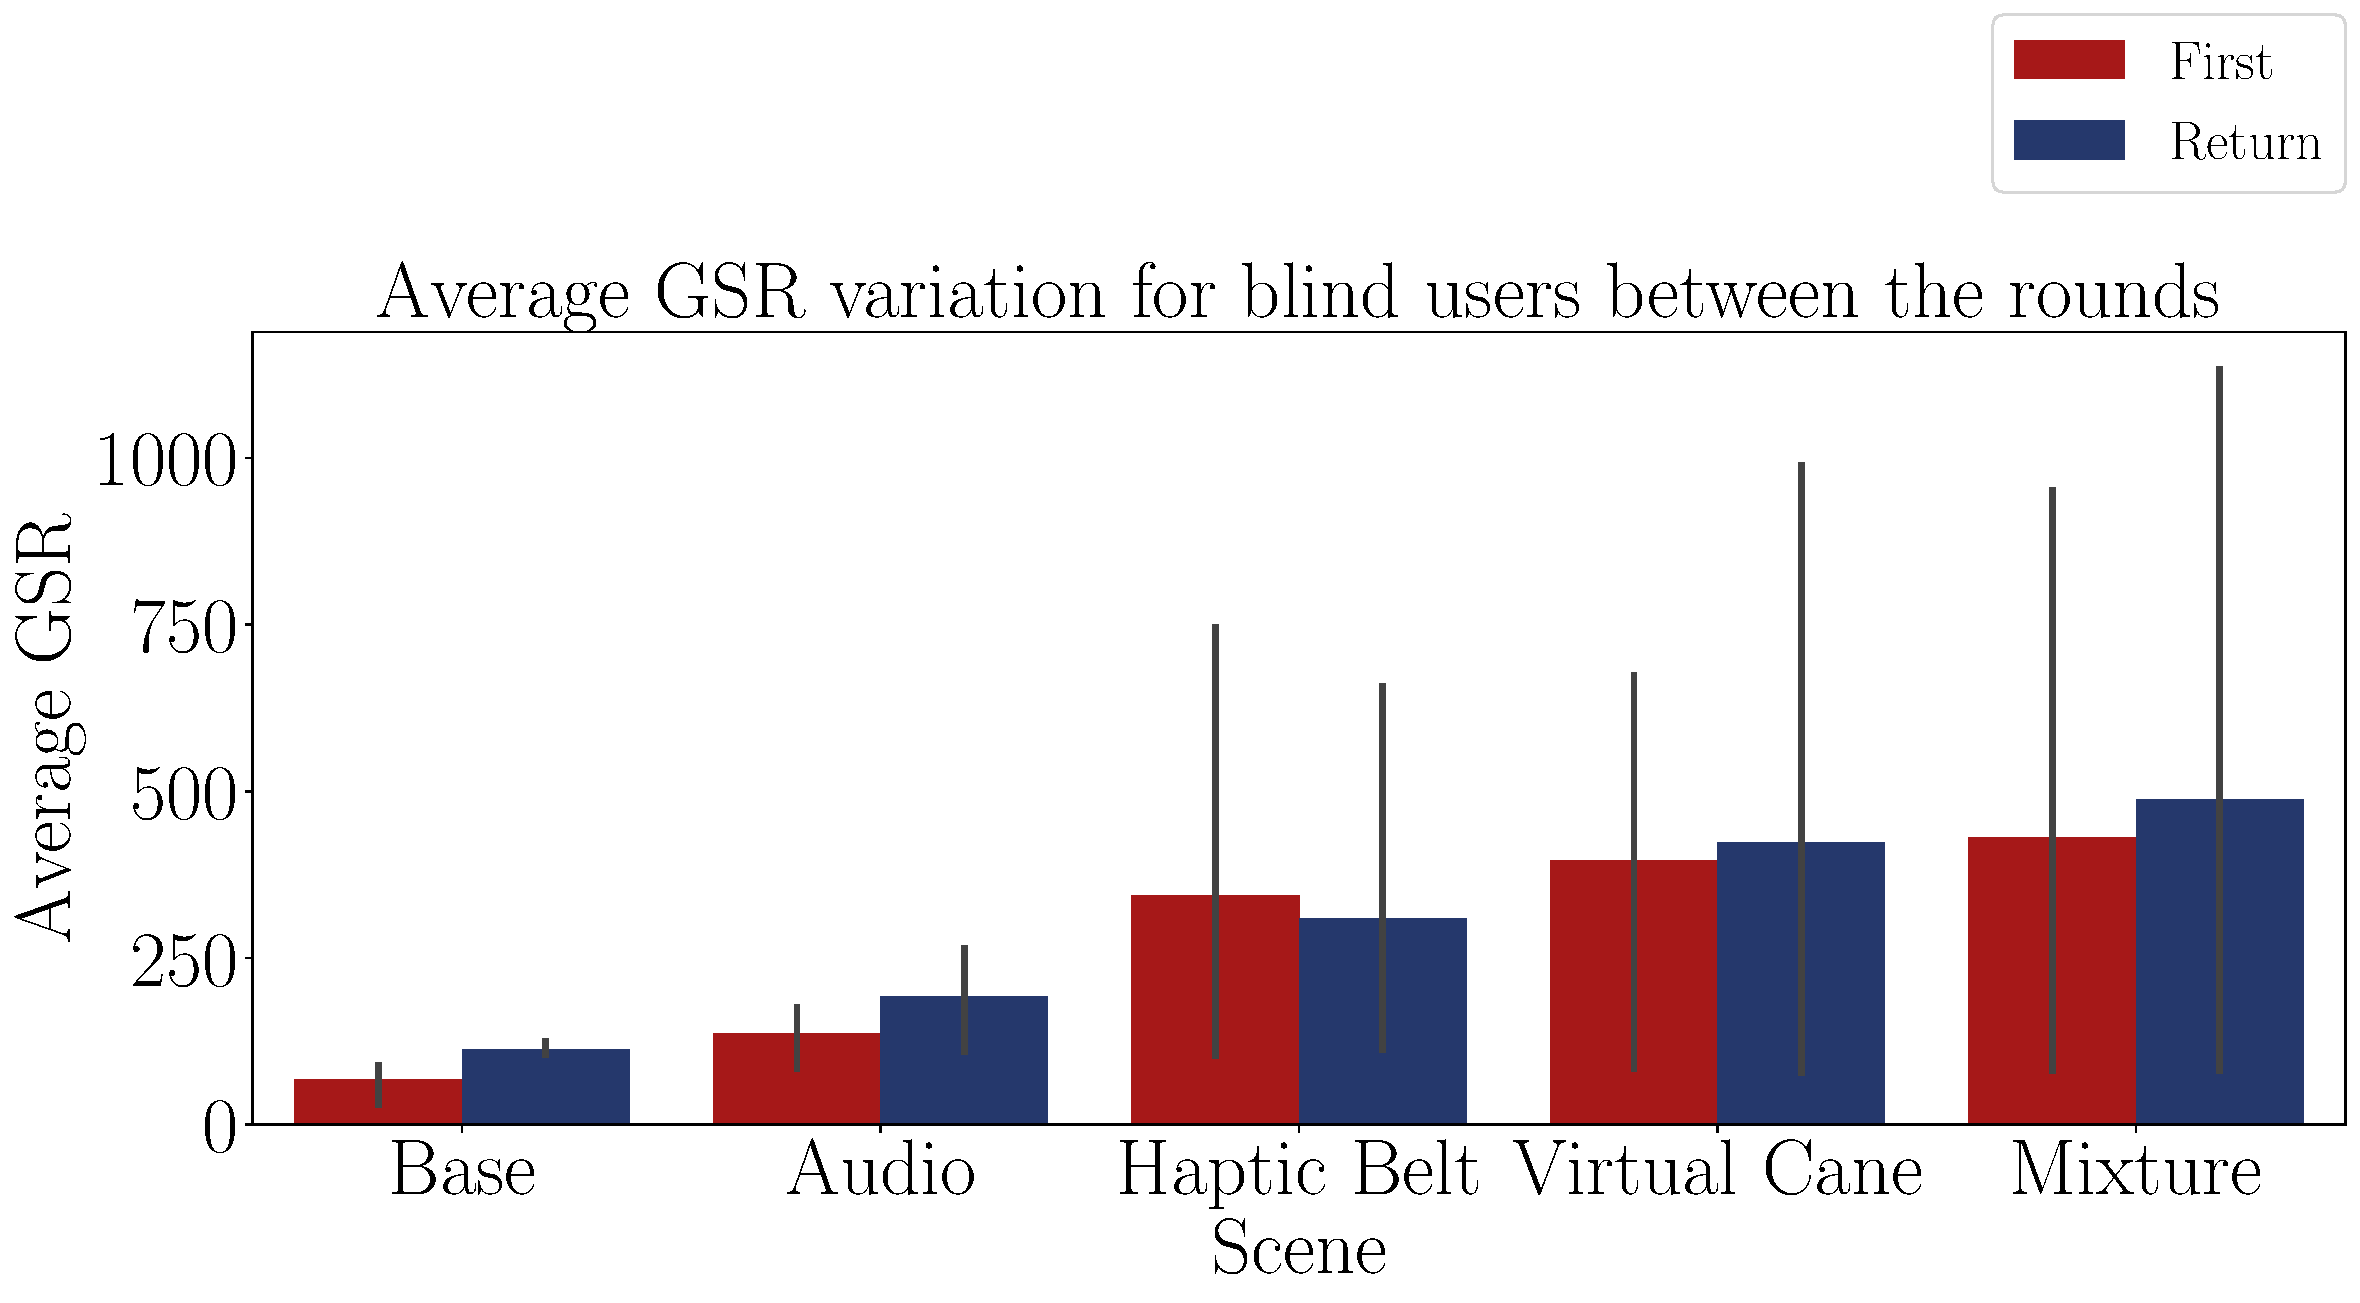
\includegraphics[width = \textwidth]{Resultados/GSR/Figuras/pdf/barplot_gsr_avg_5_scene_blind.pdf}
    \caption{Barplot of the average SDNN of the blind participants on each method.}
    \label{fig:barplot_gsr_avg_5_scene_blind}
\end{figure}

Figure \ref{fig:boxplot_gsr_avg_blind_scene} presents the boxplot of the percentual variation in the skin conductance for each method. The base method has the lowest variation among all methods. Also, the introduction of vibration increases the method variance. Figure \ref{fig:boxplot_gsr_avg_blind_rounds} presents the GSR grouped by the rounds. In this case, there is no apparent difference between the rounds.

\begin{figure}[!htb]
    \centering
    \begin{minipage}{0.45\textwidth}
        \centering
        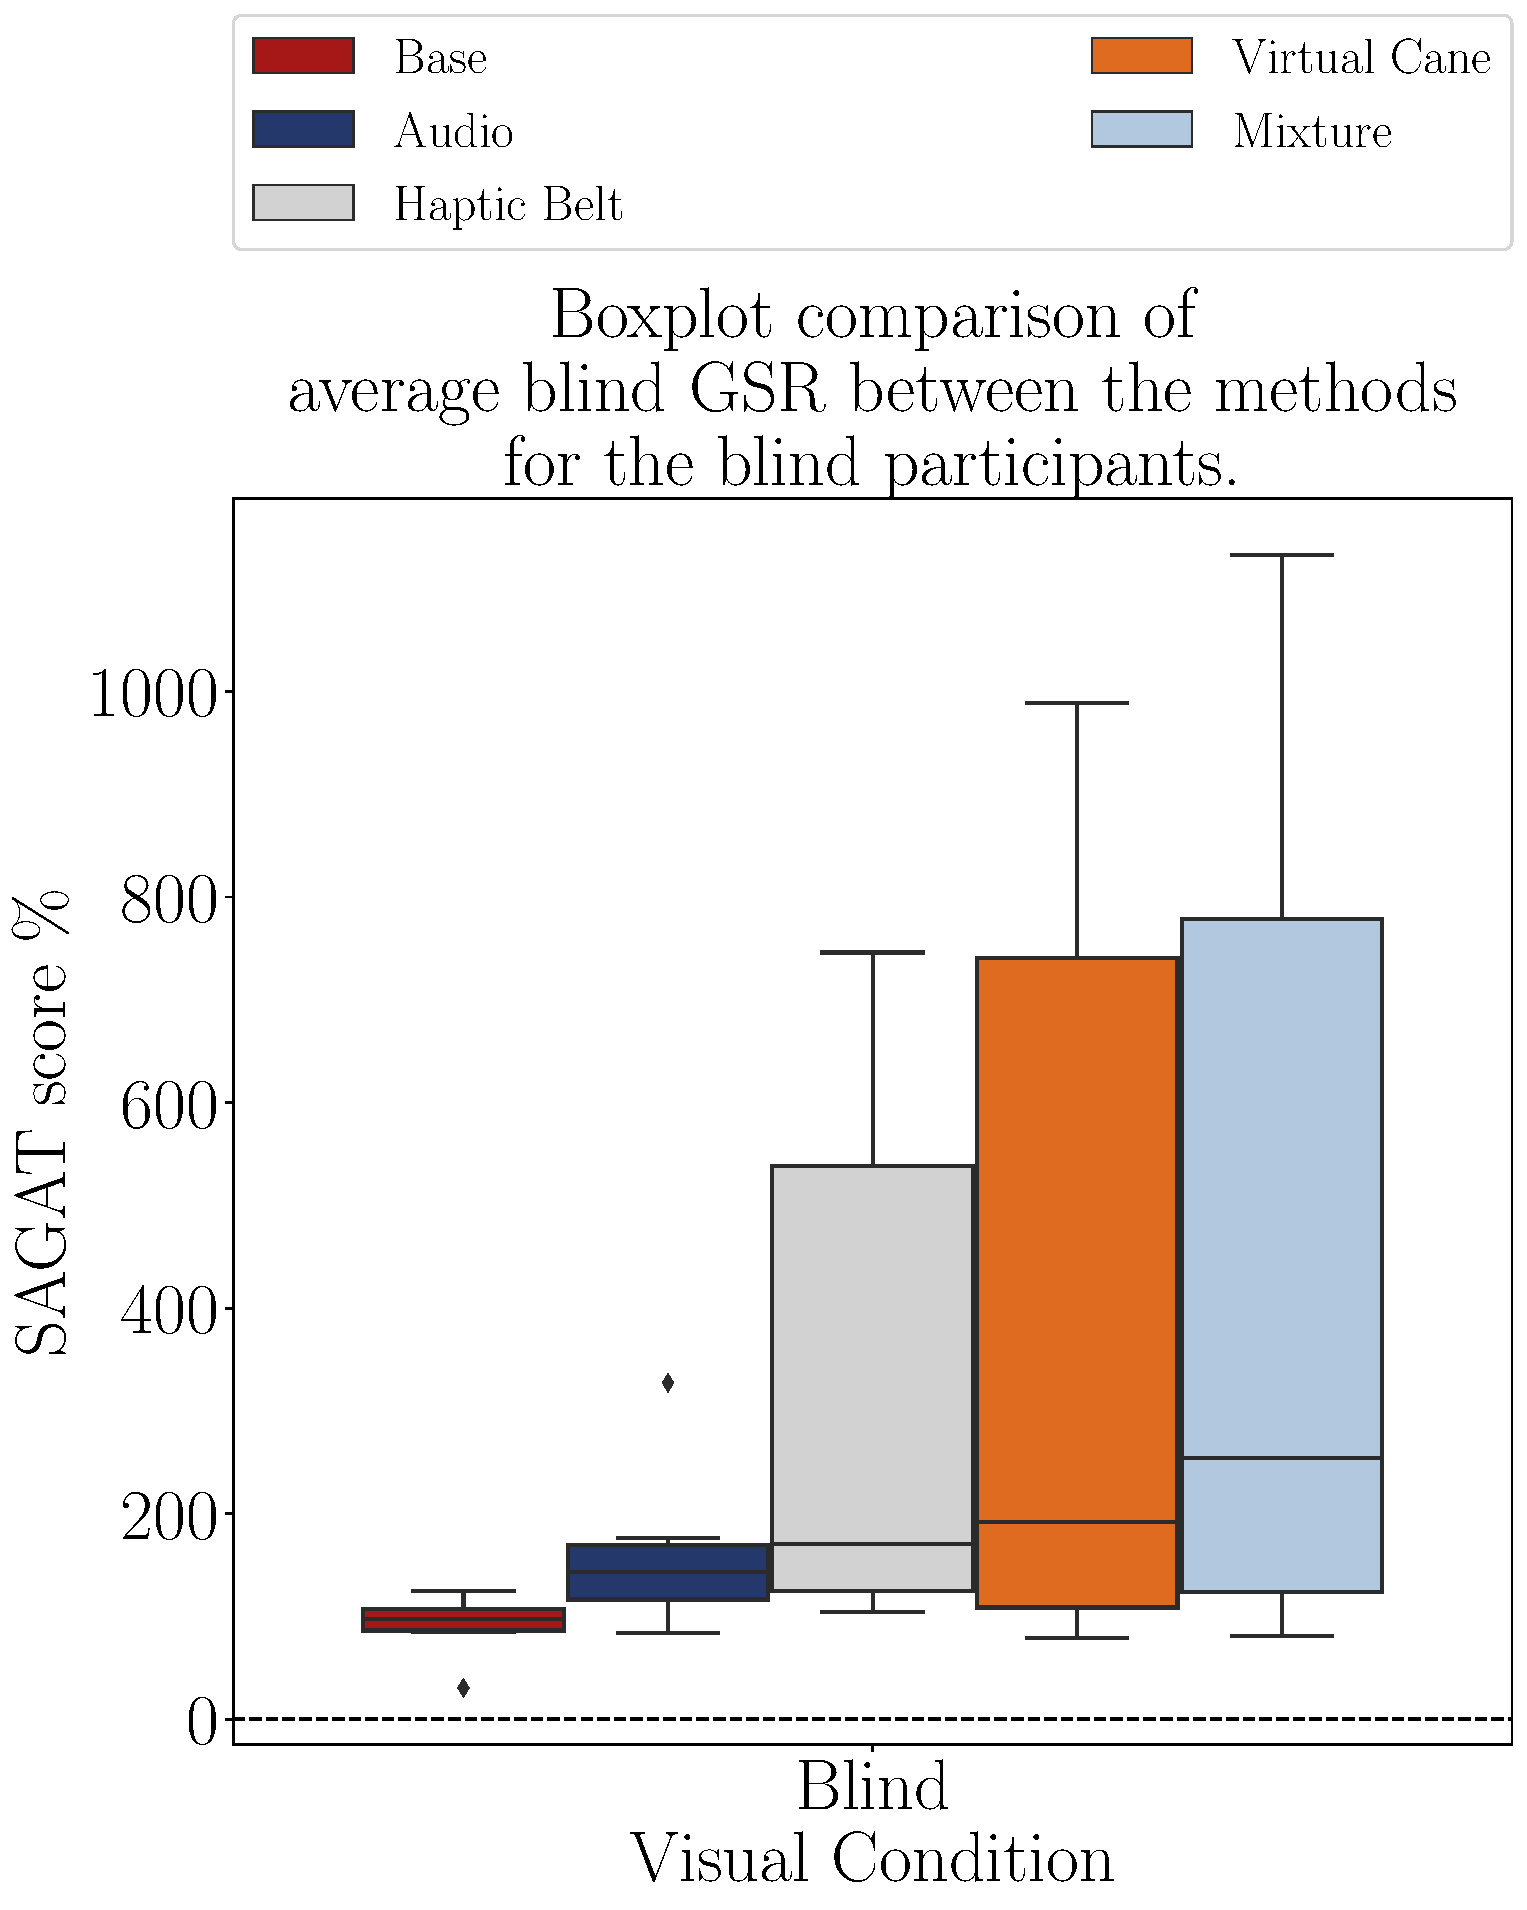
\includegraphics[width = \textwidth]{Resultados/GSR/Figuras/pdf/boxplot_gsr_avg_blind_scene.pdf}
        \caption{Boxplot of the GSR of the blind participants grouped by the methods.}
        \label{fig:boxplot_gsr_avg_blind_scene}
    \end{minipage}
    \begin{minipage}{0.075\textwidth}
        \hfill
    \end{minipage}
    \begin{minipage}{0.45\textwidth}
        \centering
        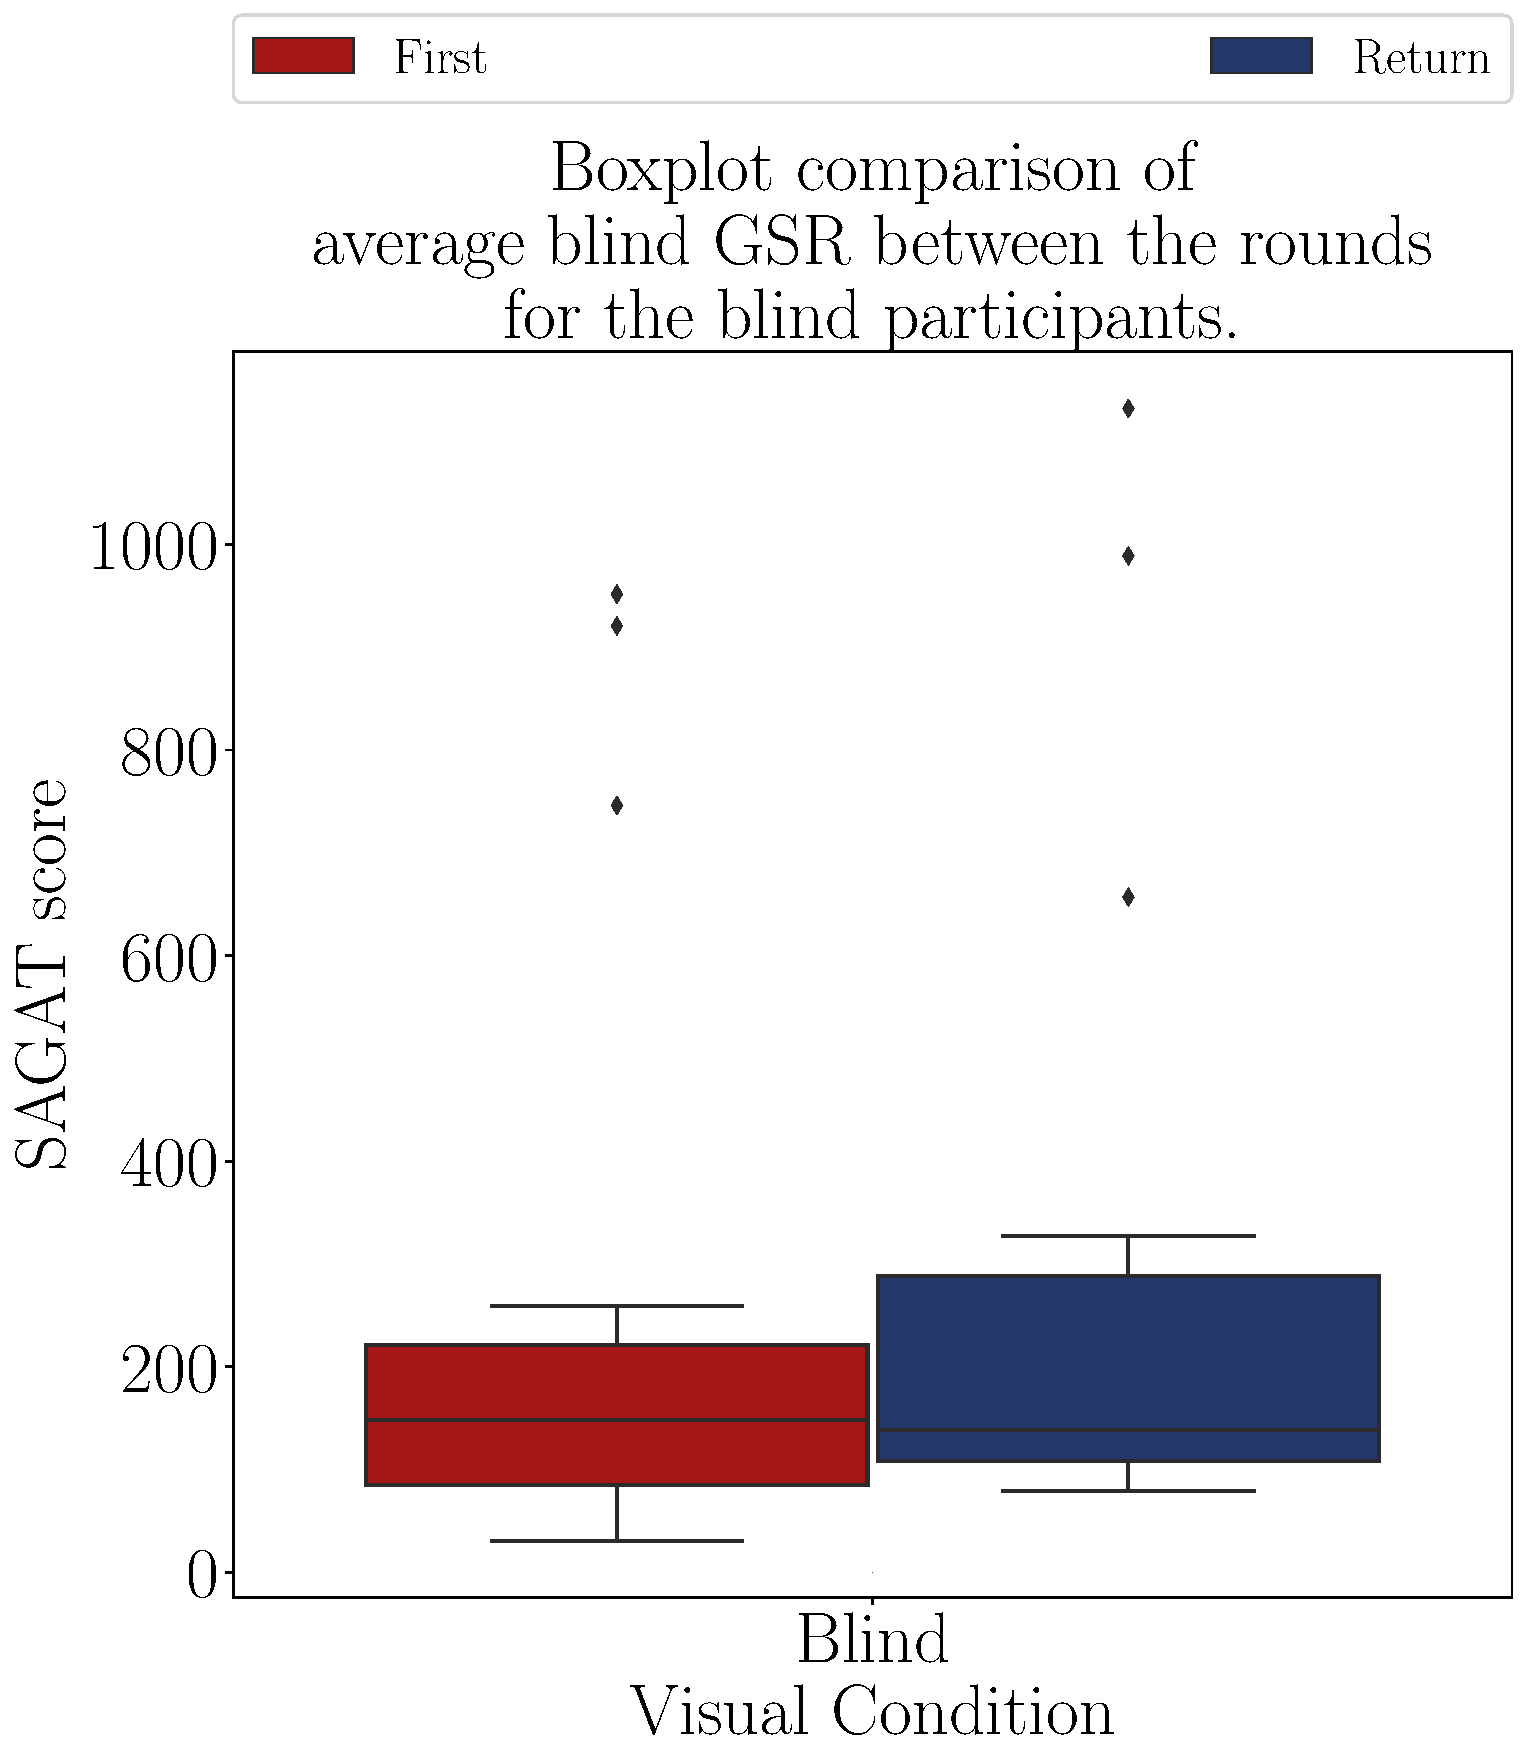
\includegraphics[width = \textwidth]{Resultados/GSR/Figuras/pdf/boxplot_gsr_avg_blind_rounds.pdf}
        \caption{Boxplot of the GSR of the blind participants grouped by the rounds.}
        \label{fig:boxplot_gsr_avg_blind_rounds}
    \end{minipage}
\end{figure}

Figures \ref{fig:qqplot_gsr_two_way_blind} and \ref{fig:residplot_gsr_two_way_blind} shows the QQ plot and the residual distribution. Table \ref{tab:blocanova_gsr_two_way_blind} shows the ANOVA test p-value for the GSR percentual variance. Although the p-value for the method is not below the threshold of 0.05, it is close to it, indicating that probably the GSR is affected by it. 

\begin{figure}[!htb]
    \centering
    \begin{minipage}{0.45\textwidth}
        \centering
        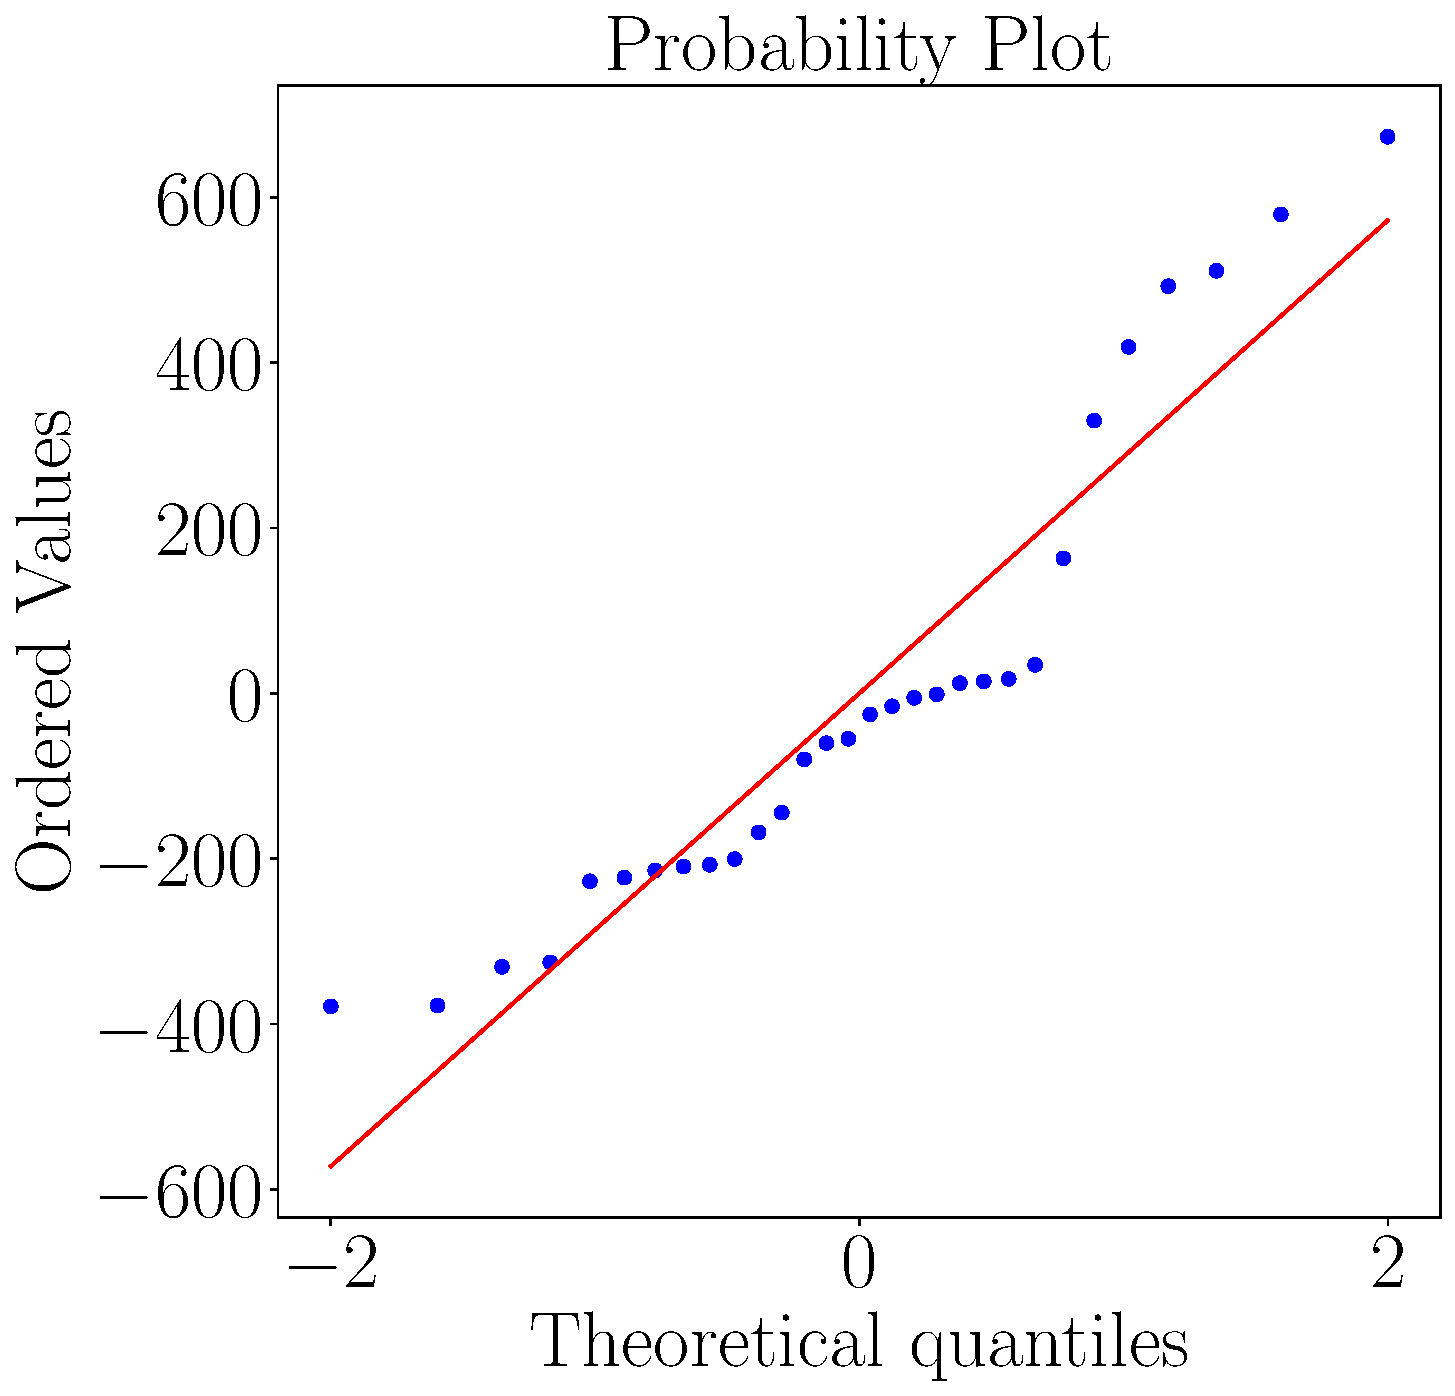
\includegraphics[width = \textwidth]{Resultados/GSR/Figuras/pdf/qqplot_gsr_two_way_blind.pdf}
        \caption{QQ plot of the SDNN of the blind participants on each method.}
        \label{fig:qqplot_gsr_two_way_blind}
    \end{minipage}
    \begin{minipage}{0.075\textwidth}
        \hfill
    \end{minipage}
    \begin{minipage}{0.45\textwidth}
        \centering
        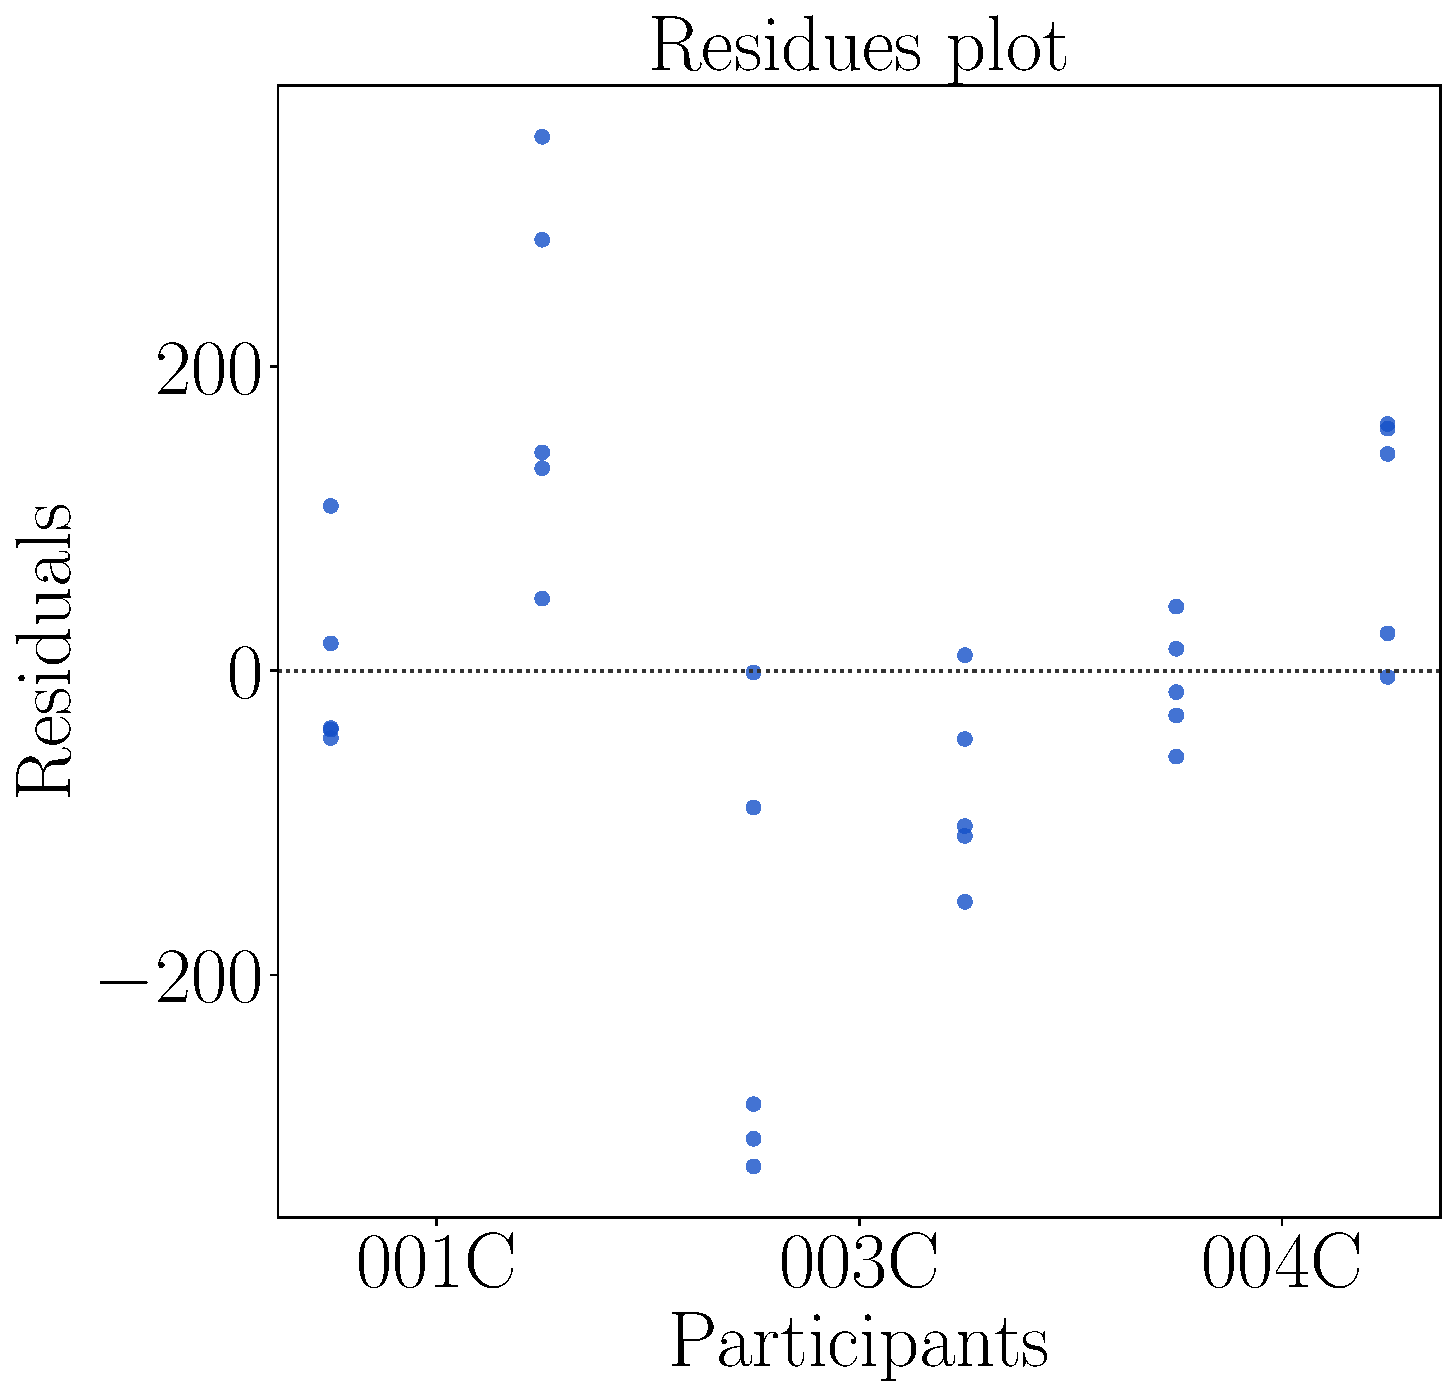
\includegraphics[width = \textwidth]{Resultados/GSR/Figuras/pdf/residplot_gsr_two_way_blind.pdf}
        \caption{Residual plot of the SDNN of the blind participants on each method.}
        \label{fig:residplot_gsr_two_way_blind}
    \end{minipage}
\end{figure}


\begin{table}[!htb]
\centering
\caption{Anova p-value for the mental demand average on each method for blinded users.}
\label{tab:blocanova_gsr_two_way_blind}
\begin{tabular}{lrrrrl}
\toprule
          Source & P-Value \\
\midrule
    \    Methods &   0.051 \\
     \    Rounds &   0.722 \\
\    Interaction &   0.996 \\
\bottomrule
\end{tabular}
\end{table}




\FloatBarrier

